%!TEX TS-program = xelatex
%!TEX encoding = UTF-8 Unicode
\documentclass{ctexart}
\usepackage[a4paper,hmargin=0.7in,vmargin=0.75in]{geometry}
\usepackage{setspace}
\usepackage{listings}
\linespread{1.5}
\newfontfamily\listingsfont{Menlo}
\lstset{lineskip={-0.5pt},breaklines,frame=single,basicstyle=\linespread{0.6}}
\usepackage[nounderscore]{syntax}
\setlength{\parskip}{1em}
\newenvironment{typewriterfont}{\ttfamily}{\par}

\title{从MiniC到RiscV \\ \large 编译实习课程报告}
\author{1500012739 特古斯}

\begin{document}
\maketitle{}
\tableofcontents
\newpage

\section{综述}

这学期的编译实习的任务是从MiniC(简化版的C)$\rightarrow$中间代码Eeyore$\rightarrow$中间代码Tigger$\rightarrow$RiscV伪汇编,每个阶段都有一定的检查以确保此阶段的正确性和进度的进展。从零开始做一个编译器的确是非常有成就感的一件事,我也在其中很大的提升了自己的代码能力。

这学期的编译实习与以往不同,第一次采用MiniC作为课程的语言平台。相对于原来的MiniJava,MiniC的语法更加简单,剔除了面向对象的内容,简化了许多的工作。但与此同时,课程设计者在课程设计也中有些缺陷和考虑欠妥的地方,经过今年的实践,我也对课程有一些建设性的提议。

\section{实验平台}

在整个实现过程中我全部采用了Lex+Yacc工具链进行翻译,因为翻译过程遵循同样的模式,修改起来也比较方便。我也曾经尝试过用Python用正则表达式匹配进行中间代码优化,不过后来由于过于繁琐还是直接用Yacc生成的代码优化了。

Yacc是一个采用LALR(1)语法分析的工具,输入BNF并添加语义规则就可以生成需要的代码,一般都要与Lex结合。Lex则是一个用正则表达式分析语言,把每个符号分解为Token进一步输入Yacc。

下面是对每个部分方法详述。

\section{MiniC}

这部分的任务是分析MiniC的语法并翻译成Eeyore。MiniC的语法比C简单了许多,不过原来的文档提供的BNF有许多漏洞,我也在基础之上加上了许多的小优化,下面是我实现的BNF。

\newpage
\subsection{BNF}
\setlength{\grammarindent}{8em} % increase separation between LHS/RHS
\begin{typewriterfont}
\begin{grammar}
<Goal> ::= DefnDeclList*

<DefnDeclList> ::= (VarDefn|FuncDefn|FuncDecl)*

<VarDefn> ::= Type Identifier ';'
\alt Type Identifier '['<INTEGER>']' ';'
\alt Type Identifier '=' Expression ';' //声明时赋值
\alt Type Identifier '['<INTEGER>']' '=' Expression ';'

<VarDecl> ::= Type Identifier
\alt Type Identifier'['<INTEGER>?']'

<FuncDefn>  ::= Type Identifier '(' ( VarDecl ( ',' VarDecl )* )? ')' '\{' (FuncDecl | Statement)* '\}'

<FuncDecl> ::= Type Identifier '(' ( VarDecl (',' VarDecl)*)?')' ';'

% <MainFunc> ::= 'int' 'main' '(' ')' '\{' (FuncDecl | Statement)* '\}'

<Type> ::= 'int'

<Statement> ::= '\{' (Statement)* '\}'
\alt 'if' '(' Expression ')' Statement ('else' Statement)?
\alt 'while' '(' Expression ')' Statement
\alt Identifier '=' Expression ';'
\alt Identifier '[' Expression ']' '=' Expression ';'
\alt Expression // 无左值表达式
\alt 'return' Expression ';'

<Expression>	::=	Expression ( '+' | '-' | '*' | '/' | '\%' ) Expression
\alt Expression ( '\&\&' | '||' | '\textless' | '==' | '\textgreater' | '!=' ) Expression
\alt Expression '[' Expression ']'
\alt <INTEGER>
\alt Identifier
\alt ( '!' | '-' ) Expression
\alt Identifier '(' (Expression (',' Expression)*)? ')' // 参数支持表达式
\alt '(' Expression ')'

<Identifier>	::=	<IDENTIFIER>

\end{grammar}
\end{typewriterfont}

\subsection{特点}

\begin{itemize}
  \item \textbf{增加了对新语法的支持}
  \begin{lstlisting}[basicstyle=\listingsfont]
  int test(){
    f(g(x) + a && b);//无返回值表达式+参数优化
    int a = 1;//直接赋值
    int g() {};//函数中定义函数
  }
  \end{lstlisting}
  与原来的BNF比较,增加了
  \begin{itemize}
    \item 无返回值表达式,如直接调用函数
    \item 表达式传入任何可传入的位置(如函数参数)
    \item 声明时直接赋值
    \item 支持在函数中声明与定义函数,作用域为最近的域。
    \item 去掉对main函数的强制要求
  \end{itemize}

  \item \textbf{对代码进行检查}
  \begin{itemize}
    \item 未声明变量或函数

    直接报错,输出出错行数并停止翻译
    \begin{lstlisting}[basicstyle=\listingsfont]
    int main(){
      t(); //Function not declared at line 2
    }
    \end{lstlisting}
    \item 重复定义变量

    采用第一次定义的变量
    \begin{lstlisting}[basicstyle=\listingsfont]
    int main(){
      int a;
      int a[100];//Ignored
    }
    \end{lstlisting}
    \item 函数参数数量不匹配

    直接报错,输出出错行数
    \begin{lstlisting}[basicstyle=\listingsfont]
    int null(int a);
    int main(){
      null(); //Function parameter error at line 3
    }
    \end{lstlisting}
    \item 语法错误

    直接报错,输出出错行数
    \begin{lstlisting}[basicstyle=\listingsfont]
    int null(int a);
    int main(){
      null(; //Syntax error at line 3
    }
    \end{lstlisting}
  \end{itemize}

\end{itemize}

\subsection{实现细节}

\begin{lstlisting}[basicstyle=\listingsfont,caption={环境结构},captionpos=b]
typedef struct environment
  {
    struct environment* pre;//前向指针
    map<string,string> symTable;//符号表
    map<string,string> declList;//已声明函数
    map<string,string> funcPara;//函数参数
    int varCnt;
  } Env;
\end{lstlisting}

\begin{figure}[htbp]
  \centering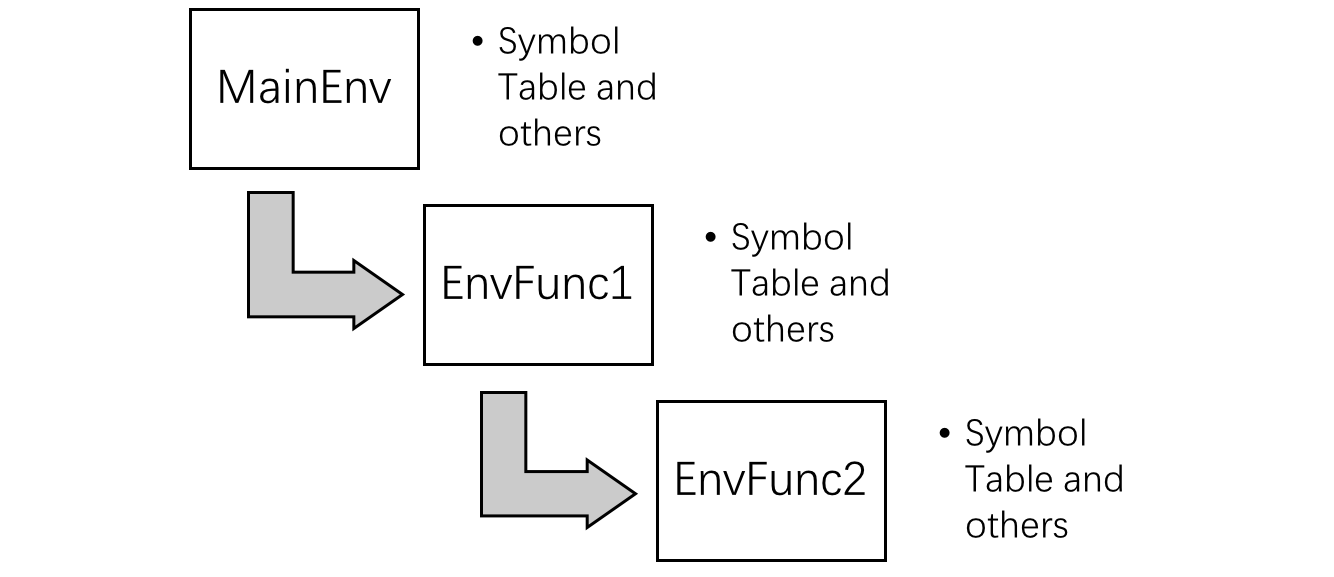
\includegraphics[width=10cm]{latexIMG/MiniCEnv.png}
  \caption{环境示意图}
  \label{}
\end{figure}

整个过程使用了On-the-fly动态生成的方法,同时考虑到并不需要特别多的依赖关系,每个非终结符号都可以用string代表它所代表的变量,整个过程非常的简洁。因为这个原因,符号表中只需存储MiniC中每个变量名和对应的eeyore临时变量名,用一个map表示符号表即可。而不同的环境用一个链表串起来,在每个环境中存储的信息只有符号表、已声明的变量集合(用来判断是否有未声明的变量)和函数参数。

对于while和if的处理,用On-the-fly生成的话非常简洁,没有回填之类的一系列问题,结构如下:
\begin{lstlisting}[basicstyle=\listingsfont]
l1:
if condition goto l2
//Loop body
goto l1
l2:

if condition goto l3
if body
l3
\end{lstlisting}

其他部分相对就简单得多,优先级我手动写了6个级别的非终结符号,但听佳晋说完全可以用left代替(捂脸)。

\subsection{编写中遇到的问题}

首先是没有理解Eeyore中变量的命名方式,一开始直接用T开头后面加乱七八糟的字母来方便调试,结果一直跑不通…才发现后面必须是标准的数字。

还有就是两方符号的识别与命名:每次识别到新的符号,直接把所有符号先转换为内部的独有变量,不过这样也带来了一些问题:对Identifier来说没有上下文信息,不好判断是在什么地方进行的,因此需要全局变量来辅助,这样也造成了一些结构上比较丑陋的地方,不过总体来说利大于弊。

为了翻译上的方便,我一开始使用了大量的临时变量存储中间结果,这也给后来的优化埋下了很多伏笔。

\subsection{实现过程中的小Tips}

因为On-the-fly生成时不存在显式的语法树,有些必须的辅助信息(如判断是否为函数参数)需要作为继承属性输入到下层的非终结符号中,而我把每个符号的类型都设置成了string……因此我就用了各种方法对栈中进行传递,比如全局变量和临时的环境。

总体来看,在MiniC翻译中用很简洁的On-the-fly生成取得了很好的效果,对代码错误也有一定的查错能力,不过生成的Eeyore代码还有很多的冗余,这将在之后的中间代码过程中逐步进行优化。

\subsection{尚待改进之处}

一个挺大的缺陷就是不支持短路表达式和++符号。短路表达式是非常有趣的一个内容,由于时间限制没有完成;++符号在生成代码时的顺序问题也是很精妙的。还有就是没有完成类型检查,对于强类型语言来说有一点缺陷。

\section{Eeyore}

从Eeyore翻译到更底层的Tigger是整个编译器的核心。在这个过程中,我们需要进行Eeyore代码的翻译和优化,并进行寄存器分配,最终生成Tigger代码。

这阶段最大的挑战是要初步分析出每个函数的栈空间、将无限的变量分配到有限的寄存器和代码更细粒度的分解。
\newpage
\subsection{BNF}
因为需要能在Eeyore模拟器上正确运行,这里的BNF和原来没有什么变化。
\begin{typewriterfont}
\setlength{\grammarindent}{8em} % increase separation between LHS/RHS
\begin{grammar}
<Declaration> ::= 'var' <INTEGER>? Variable

<FunctionDecl> ::= Function '[' <INTEGER> ']' '\textbackslash n' ((Expression | Declaration)'\textbackslash n')* 'end' Function

<RightValue> ::= Variable | <INTEGER>

<Expression>	::=	Variable '=' RightValue OP2 RightValue
\alt Variable '=' OP1 RightValue
\alt Variable '=' RightValue
\alt Variable '[' RightValue ']' = RightValue
\alt Variable = Variable '[' RightValue ']'
\alt 'if' RightValue LogicalOP RightValue 'goto' Label
\alt 'goto' Label
\alt Label ':'
\alt 'param' RightValue
\alt Variable '=' 'call' Function
\alt 'return' RightValue


<Identifier>	::=	<IDENTIFIER>

<Variable> ::= <VARIABLE>

<Label> ::= <LABEL>

<Function> ::= <FUNCTION>

\end{grammar}
\end{typewriterfont}

\subsection{特点}

\begin{itemize}
  \item 采用线性扫描的寄存器分配算法
  \item 运用了多项优化手段
  \item 某些寄存器分配了特定的用途
\end{itemize}

\subsection{实现}

相对于原来复杂的语法树,Eeyore代码没有显式的多层嵌套,只有在分支的时候有两种分叉。在分析Eeyore代码时直接将代码存为链式结构,并存储可能的后继,之后再对整个代码数组进行分析即可。

生成内部表示代码的数组之后,对每一个函数进行活性分析,产生每个变量的活跃区间,然后对代码进行优化,得到优化后的代码后用线性扫描进行寄存器分配,最终生成Tigger代码。

\begin{lstlisting}[basicstyle=\listingsfont,caption={变量结构},captionpos=b]
struct variable{
  int id,st,ed,isGlobal,isArray,glbID;\\从Eeyore文件中分析得出
  int _pos,_reg,_mem,_active;\\在活性分析中用到
  int pos,reg,mem,active;\\在代码生成中用到
  string name;

  variable(string _name,int _id,int memID = 0):id(_id),name(_name)\\构造函数
  {
    mem = memID;isArray = 0;
    st = 63333;ed = -1;_pos = 0;_reg = 0;
    if(mem == 0) {isGlobal = 1;glbID = glbID_cnt++;}
    else isGlobal = 0;
  };
  variable() {};
};
\end{lstlisting}
\begin{lstlisting}[basicstyle=\listingsfont,caption={代码块结构},captionpos=b]
struct block{
  int type;\\代码类型
  string arg1, arg2, arg3, arg4;\\不同参数
  vector<int> pre;\\语句的前驱
  bitset<MAXVARS> def,use,live;
  block(int _type, string _arg1 = "", string _arg2 = "", string _arg3 = "", string _arg4 = ""):
  type(_type),arg1(_arg1),arg2(_arg2),arg3(_arg3),arg4(_arg4) {};
};
\end{lstlisting}
\begin{lstlisting}[basicstyle=\listingsfont,caption={函数结构},captionpos=b]
struct myfunction{
  string name;
  int stackSize,varCnt;\\变量数和栈空间
  myfunction(string _name,int _varCnt)
  {
    name = _name;
    varCnt = _varCnt;
    stackSize = 12;
  };
  myfunction(){};
};
\end{lstlisting}

\subsection{活性分析}

我做的是关于函数域中的活性分析。首先要分析出代码的结构以确定每个语句的前驱与后继,这里除了if有两个后继,goto有确定的后继,其它都是确定的一个后继。这样我们就可以计算出每个语句的前驱和后继,之后从最后一条语句开始计算live变量(用bitset存储),有改变的话就把前驱放在queue中,用一个类似BFS的算法不断遍历,直到queue中没有语句为止,也就是收敛了。确定了每个语句的活跃变量之后,我直接粗暴地把每个变量的活跃区间设为最前面活跃到最后活跃的长度(否则会造成非常麻烦的情况,课上也讨论过这个问题)。

\subsection{优化代码}

总的来说这部分很多是给之前Eeyore填坑……我的优化步骤是:单步窥孔优化$\rightarrow$复写传播$\rightarrow$无用代码消除$\rightarrow$if表达式优化$\rightarrow$代码外提$\rightarrow$表达式计算。其中每个步骤我都是把每条语句看作单独的基本块,复杂度上来说也是够用的。

\begin{itemize}
  \item 窥孔优化:前一步生成的代码有许多$b = a, c = b$性质的语句;我的处理方法是是判断b的活跃区间是否只在这两句话,如果是的话直接删除并替换即可;
  \begin{lstlisting}
  T1 = a + b;
  T2 = T1;
  优化前
  T1 = a + b;
  T2 = T1;
  优化后
  \end{lstlisting}
  \item 复写传播:对每条赋值的语句,在一个基本块中之后对其def之前所有变量用其左值替换,为给之后死代码消除提供空间;(保证正确性在基本块中优化即可)
  \begin{lstlisting}
  T1 = T2;
  T3 = T1;
  优化前
  T1 = T2;
  T3 = T2;
  优化后
  \end{lstlisting}
  \item 无用代码消除:此处描述的无用代码代表两层含义:一是没有use过的变量,二是goto等造成的不可能执行的表达式。对于情况一,直接用活跃区间判断即可(上面的复写传播也会给优化提供空间);情况二将goto代码进行分析,goto后面的到label之间的代码可以直接删除。
  \begin{lstlisting}
  a = 2
  goto l2
  blablabla
  l1
  优化前
  goto l2
  l1
  优化后
  \end{lstlisting}
  \item if表达式优化:同样是优化前一步Eeyore生成的坑,原本在if中只有$if a == 0 goto$类型的,在这里把逻辑表达引入了if语句之中,节省了代码数量和寄存器
  \begin{lstlisting}
  T1 = T2 < T3
  if T1 == 0 goto l2
  优化前
  if T2 >= T3 goto l2
  优化后
  \end{lstlisting}
  \item 表达式计算:如果一个表达式是二元或单元常数运算,那么编译器直接算出来就可以
  \begin{lstlisting}
  T1 = 1 * 4
  优化前
  T1 = 4
  优化后
  \end{lstlisting}
  \item 代码外提:对循环不变量的外提也是重要的一个步骤。我的方法算是初步的数据流分析(山寨版)
  \begin{itemize}
    \item 首先是要生成每个基本块的ud链:方程:$$in[B] = \cup_{pre} out[B], out[B] = gen[B] \cup (in[B] - kill[B])$$其中gen和kill代表每一句生成的语句和失效的表达式,这里因为基本块以语句为单位,gen就为本身,kill为定义了此语句左值的所有语句。用bitset记录各个值,与活性区间相似的方法迭代得出ud链。
    \item 之后提取循环块:用模式匹配方法:从label到对应的goto代表一个循环,得出循环块。这样得出的循环在循环嵌套中是由大到小的,从父级块中先提取。
    \item 但是如果要把每一个不变量都提出去的话,会是非常麻烦的操作。为了保证正确性,我只考虑了define都在循环之外的语句:分析每一个语句的ud链,若全部在循环体之外,则将它移到循环之前。
  \end{itemize}

  \begin{lstlisting}[basicstyle=\listingsfont,caption={函数结构},captionpos=b]
  for(int i = 0;i < blocks.size();i++)
  {
    int end = -1;
    if(blocks[i].type == iLABEL)
    {
      for(int j = i + 1;j < blocks.size();j++)
      {
        if(blocks[j].type == iGOTO && blocks[j].arg1 == blocks[i].arg1)
        {
          end = j;
          break;
        }
      }
    }//找出循环块(保证循环块结构是一个模式)
    if(end == -1)
    continue;
    for(int j = i;j < end;j++)
    {
      int flag = 0;
      for(int k = i;k < end;k++)
      {
        if(blocks[j].ud_chain[k]) flag = 1;
      }
      if(flag == 0)
      {
        block tmp = blocks[j];
        blocks.erase(blocks.begin() + j);
        blocks.insert(blocks.begin() + i,tmp);
      }
    }//不变量外提
  }
  \end{lstlisting}
\end{itemize}

\subsection{寄存器分配}

现在大家主要都是采用的线性扫描算法,与原本的图染色相比代码好写了许多,性能根据观察也没有很大的损失,同时性能也有很大提高($O(n)$)。具体的算法如下:

根据活跃区间结束位置排序,贪心地将每个寄存器分配给相应的变量,当变量不活跃时释放寄存器,给下一个变量留出空间。如果需要溢出,找到其中起点最早的变量,对它进行溢出,将寄存器分配给新变量即可。然而由于寄存器非常的多,构造复杂的例子还是很难的。

在RiscV的23个可用寄存器中,为了提高性能和解决奇怪的Tigger语法问题(Reg和Immediate计算),我将三个寄存器固定了用途:
\begin{itemize}
  \item s8专门存储数字4,处理数组地址问题(取值时都会乘4)
  \emph{后面用位移运算改进了,完全可以不需要这一个,但是Tigger模拟器不能做相乘的操作就保留了下来}
  \item s9专门存储立即数1,做与寄存器的二元运算
  \item s10专门存储立即数2,做与寄存器的二元运算(其实可以删除因为立即数与立即数计算已经被优化了)
  \item s11专门存储临时的地址,处理数组地址问题
\end{itemize}

\subsection{代码生成}
理论上直接把每个代码按规则翻译就好了……但是写代码的时候这时候出的Bug最多。

问题主要出在寄存器的分配。虽然每个变量对应寄存器有了,但是对应到每个语句就需要判断是否应该load或store。我的方法是就是线性扫描代码,在扫描过程中保存每个变量和寄存器的状态(如上面的结构体),并根据变量是否活跃的状态store/load相应的寄存器。

另外的困难就是调用函数时对栈帧的处理。调用函数时,记录之前的param命令,将caller-saved寄存器的值load到内存/栈中,然后把参数传到寄存器中(顺序不能变化)。每个函数开头还需要保存callee-saved寄存器,为了减小开销我们都只是保存/恢复活跃的寄存器。其他的细节都在代码里,在此就不再赘述了。

\subsection{优化效果}
这里我使用了自己写的qsort和原本课程设计者提供的wseq,分别统计优化前和优化后的Tigger代码长度和运行时用translate得出的实际指令数。

\begin{center}
  \begin{tabular}{cccccccc}
  \hline
  源文件& Tigger优化前& Tigger优化后& RiscV优化前& RiscV优化后& Tigger模拟器运行时间\\
  \hline
  qsort& 271& 236& 48608& 48490& 1.49->1.07\\
  wseq& 459& 434& -& -& -\\
  \hline
  \end{tabular}
\end{center}


wseq测试量过大,没有实际在模拟器上测试。RiscV实际运行指令数相对改进不大的缘故,应该是运行时环境占了大多数指令(尤其是系统调用的printf函数什么的)。总体来看优化还是能起到比较显著的效果。
\section{Tigger}

从Tigger到RiscV相对来说比较简单,我实现的是32位版本的RiscV,指针和int大小是一样的,带来了很多方便。根据表格提供的代码一条一条翻译过去就好。有一些命令没有提供,我填补之后的结果附在了后面。

\newpage
\subsection{BNF}

\begin{typewriterfont}
\begin{grammar}
<Goal>  ::= (FunctionDecl | GlobalVarDecl)*

<GlobalVarDecl> ::= <VARIABLE> '=' <INTEGER>
\alt <VARIABLE> '=' 'malloc' <INTEGER>

<FunctionDecl> ::= Function '['<INTEGER>']' '['<INTERGER>']' (Expression)* 'end' Function

<Expression>	::=	Variable '=' Reg OP2 Reg
\alt Reg '=' Reg OP2 <INTEGER>
\alt Reg '=' OP1 Reg
\alt Reg '=' Reg
\alt Reg '=' <INTEGER>
\alt Reg '[' <INTEGER> ']' = Reg
\alt Reg = Reg '[' <INTEGER> ']'
\alt 'if' Reg LogicalOP Reg 'goto' Label
\alt 'goto' Label
\alt Label ':'
\alt 'call' Function
\alt 'store' Reg <INTEGER>
%\alt 'store' Reg <VARIABLE>
\alt 'load' <INTEGER> Reg
\alt 'load' <VARIABLE> Reg
\alt 'loadaddr' <INTEGER> Reg
\alt 'loadaddr' <VARIABLE> Reg
\alt 'return'

<Reg> ::= 'x0'
| 's0'
| 's1'
| 's2'
| 's3'
| 's4'
| 's5'
| 's6'
| 's7'
| 's8'
| 's9'
| 's10'
| 's11'
| 'a0'
| 'a1'
| 'a2'
| 'a3'
| 'a4'
| 'a5'
| 'a6'
| 'a7'
| 't0'
| 't1'
| 't2'
| 't3'
| 't4'
| 't5'
| 't6'

<Label> ::= <LABEL>

<Function> ::= <FUNCTION>

\end{grammar}
\end{typewriterfont}

\begin{table}[ht]
\caption{翻译表}
\label{my-label}
\begin{center}

  \begin{tabular}{|l|l|}
  \hline
  function {[} int1 {]} {[} int2 {]} & \begin{tabular}[c]{@{}l@{}}.text\\ .align 2 \\ .global function \\ .type @function,\\ function: \\ add sp,sp,-stk\\ sw ra stk-4(sp)\\ stk = ( int2 / 4 +1 ) * 16\end{tabular} \\ \hline
  end function & \begin{tabular}[c]{@{}l@{}}.size function, .-function\\ stk = 0\end{tabular} \\ \hline
  global\_var = malloc int & .comm global\_var,int*4,4 \\ \hline
  global\_var = int & \begin{tabular}[c]{@{}l@{}}.global v0 \\ .section .sdata \\ .align 2 \\ .type v0, @object \\ .size v0, 4,\\ v0:\\ .word int\end{tabular} \\ \hline
  reg = integer & li reg,integer \\ \hline
  reg1 = reg2 op reg3 & op reg1,reg2,reg3 \\ \hline
  \&\& & \begin{tabular}[c]{@{}l@{}}seqz reg1,reg2\\ add reg1,reg1,-1\\ and reg1,reg1,reg3\\ snez reg1,reg1\end{tabular} \\ \hline
  || & \begin{tabular}[c]{@{}l@{}}or reg1,reg2,reg3 \\ snez reg1,reg1\end{tabular} \\ \hline
  != & \begin{tabular}[c]{@{}l@{}}xor reg1,reg2,reg3 \\ snez reg1,reg1\end{tabular} \\ \hline
  reg1 = reg2 & mv \\ \hline
  reg1 {[} int {]} = reg2 & sw \\ \hline
  reg1 = reg2 {[} int {]} & lw \\ \hline
  if reg1 op reg2 goto Label & op reg1,reg2,.label \\ \hline
  goto label & j label \\ \hline
  label: & .label: \\ \hline
  call function & call function \\ \hline
  store reg int & sw reg,int*4(sp) \\ \hline
  load int reg & lw reg,int*4(sp) \\ \hline
  load global\_var reg & \begin{tabular}[c]{@{}l@{}}lui reg,\%hi(global\_var)\\ lw reg,\%lo(global\_var)(reg)\end{tabular} \\ \hline
  loadaddr int reg & add reg,sp,int*4 \\ \hline
  loadaddr global\_var reg & \begin{tabular}[c]{@{}l@{}}lui reg,\%hi(global\_var)\\ add reg,reg,\%lo(global\_var)\end{tabular} \\ \hline
  return & \begin{tabular}[c]{@{}l@{}}lw ra,stk-4(sp)\\ add sp,sp,stk\\ jr ra\end{tabular} \\ \hline
  \end{tabular}
\end{center}
\end{table}

\subsection{实现细节}

在翻译过程中我发现用移位操作代替乘法能够减小指令强度,尤其是对于大量对数组地址乘4.于是我直接采用了slli左移两位代替。不过现在我对RiscV的基本指令还不是特别理解,伪指令在手册中并没有特别多的说明,还需要自己发掘基本指令的关系,希望以后的课程上可以稍微增多讲解。

\section{测试}

编译器完成后麻烦的是各种测试…首先课程设计者提供了一部分测试代码,不过有一些问题:

\begin{itemize}
  \item 首先是代码规范和原来的不一致,在修改了BNF之后才能够正确运行
  \item 样例数据量太大,wseq在Tigger模拟器上跑需要数十分钟
  \item 没有标准的Eeyore和Tigger代码作参考,给调试造成了一些不便
\end{itemize}

我使用了自己写的一版qsort进行初步评测,代码如下。在测试中遇到的问题在解决之后很多都不记得了……一般都是自己的小Bug或功能不完善造成的。

\subsection{一些有趣的Bug}
\begin{itemize}
  \item 传参顺序问题
  在param时把变量加载到寄存器中的操作要放在最后,否则就有可能出现变量加载无效的情况
  \item Spill和GetReg会出奇怪的事情
  最主要解决的还是这部分的各种问题,不该处理的Spill,该处理的没有Load什么的……我花费了很多精力在这部分的处理
  \item 环境问题
  Mac下能通,Linux下出现问题。问题是某些变量初始化Linux默认非零;有些环境下Yacc和Bison支持的特性不一样,会出现编译错误。
\end{itemize}

\begin{lstlisting}[basicstyle=\listingsfont]
int a[10000];
int c;
int getint();
int putint(int x);
int display(int array[100], int n)
{
    int i;
    int o;
    i = 1;
    while (i < n + 1) {
      int x;
      x = array[i];
      o = putint(x);
      i = i + 1;
    }
    return 1;
}

int quicksort(int array[100], int maxlen, int begin, int end)
{
    int i;
    int j;
    if(begin < end)
    {
        i = begin + 1;
        j = end;
        while(i < j)
        {
            if(array[i] > array[begin])
            {
                int t;
                t = array[i];
                array[i] = array[j];
                array[j] = t;
                j = j - 1;
            }
            else
            {
                i = i + 1;
            }
        }
        if(array[i] > array[begin] - 1)
        {
            i = i - 1;
        }

        int t;
        t = array[begin];
        array[begin] = array[i];
        array[i] = t;

        int o;
        o = quicksort(array, maxlen, begin, i);
        o = quicksort(array, maxlen, j, end);

        return 1;
    }
    else {
      return 1;
    }
}

int main()
{
    int n;
    int array[10000];
    n = getint();
    int i;
    i = 1;
    while (i < n + 1) {
      array[i] = getint();
      i = i + 1;
    }

    int o;
    o = display(array, n);

    int st;
    st = 1;
    int ed;
    ed = n;
    o = quicksort(array, n, st, ed);
    o = display(array, n);
    return 0;
}
\end{lstlisting}

\subsection{对测试样例的建议}
\begin{itemize}
  \item 提供充足的小样例
  我在一开始做的时候完全是一头雾水,lex和yacc如何使用都不清楚,而且要把完整的语法实现出来再调试都非常困难。所以提供几个个小样例和对应的Eeyore代码在模拟器中对拍,让同学入门会比较方便。
  \item 全面完善样例
  在自己测试过程中突然发现了一个问题——机测上能通过的代码本地却有问题:纠结了一番发现是函数传递数组的问题,这个特性在原来的MiniC中存在,然而机测中并没有发现……我的建议是直接把sort里面的数组放在函数中传递。还有多寄存器的问题现在的样例做的比较简陋(直接用26个赋值语句解决问题)。
\end{itemize}

\section{对课程的建议}
毕竟是第一年的课程改革,这学期的课程的确有一些不完善之处。但总体来说在老师和助教的帮助下,整个过程还是非常顺利完成了。

\subsection{关于开发环境}
现在很大的问题是测试与开发环境的融合。辛苦助教了一学期用原始的FTP+脚本+邮件进行测试,对教学双方都不是很方便。每节课很多时间都是浪费在同学与助教交流如何测试和测试结果之类的问题,消耗了大量的时间。

一开始就碰到了Mac和Linux环境下makefile的问题,Mac下正常运行的Linux却不通过,后来研究是编译选项的问题,然后又在文件输入输出统一上浪费了很多时间与精力。

我的建议是统一一下测试环境,在实验室机器上提供独立的Docker或独立的账户供同学们使用。然后在测试上希望写一个Web端的平台让同学们提交tar包就可以,并将结果实时反馈出来,还可以增加排行榜提高课程的趣味性。尤其是提供小样例能给对某个特定功能差错或优化提供更大的便利。

\subsection{关于模拟器}
总体来说模拟器还是非常优秀的,没有遇到特别大的问题。遇到的问题一个是对大数组的处理不太好,有时候会使程序崩溃;其二是对逻辑运算符的支持有一点问题,使用Tigger输入小于等于号的话会有错误的发生。其三是Eeyore里面的param不能传递立即数。

\subsection{其它感想}
和老师的交流了很多,主要想法还是加强与理论课的联系。理论课的进度和实习课不大相符,主要有难度的寄存器分配部分理论课没有过多讲解,编译器的前端理论课上花了很多精力讲解。

然后有可能调整一下进度:目前前端部分相对来说比较简单,而留给大家的时间稍微长了些,可以在第一个月就尽量做完,重点放在中间代码部分,并在课上给大家细致地讲解。

\section{个人收获}
从0开始到完整的编译器的过程充满了艰辛,同时也学到了很多。
\begin{itemize}
  \item 付诸理论于实践

  曾经学习编译原理主课的时候,对于后半部分的代码优化和SDT没有很明白,很多题目不用遵循严格的算法都可以做出来,而到了真正的实践中必须遵循严谨的步骤。尤其是每一步的数据流分析,学习的时候并没感受到特别的意义,而在优化中它的功能是无比强大。变量的活性分析和其它优化都依赖着不同分析方法得出的结果,而其中的细微差别在实践中才能更好地理解。

  \item 提升编程能力

  把各个部分代码加起来大约有2400行,如此大的工程量可以说是前所未有的大挑战。还需要熟悉每个工具的功能,将不同模块抽象化,将细小的部分拼接在一起,查找一个符号的小Bug……第一次体验到大工程的感觉。尤其是其中的Eeyore$\rightarrow$Tigger部分,让我Debug能力得到了大幅提高。在这个过程中写bash脚本、使用git、makefile等工具我也初识了门道。

  \item 合作与讨论

  实习课课上风格也画风迥异,老师的讲解并不多,而是以同学们自主交流为主。在和同学、老师、助教讨论之后,许多不理解的问题也有了一些思路,编写代码过程中也参考了同学、助教的许多思路。在这里非常感谢给予我许多帮助的老师同学,蔡佳晋、陈梓立、肖博文等等。

\end{itemize}
\end{document}
